\documentclass[10pt]{article}

\usepackage[margin=1in]{geometry}
\usepackage{amsmath}
\usepackage{booktabs}
\usepackage{threeparttable}
\usepackage{caption}
\usepackage{graphicx}
\usepackage{newpxtext,newpxmath}
\usepackage{url}
\usepackage{xcolor}
\usepackage{tikz}
\usetikzlibrary{arrows.meta, positioning, calc, fit, backgrounds}
\usepackage[colorlinks=true,allcolors=blue]{hyperref}

\graphicspath{{figures/}}

\title{Do Lesion-Focused Inputs Improve Skin Cancer Classification Under Domain Shift?}
\author{Tobias Roemer, Thomas Lee, and Leo Li}
\date{}

\begin{document}

\maketitle

\begin{abstract}
Deep learning classifiers for skin cancer can reach dermatologist-level accuracy on standardized dermoscopic benchmarks, yet they often degrade sharply when applied to images from different cameras, clinical settings, or patient populations\,---\,a brittleness sometimes attributed to background shortcuts the model learns rather than lesion-specific features. In this light we ask: do skin lesion classifiers therefore generalize better when their inputs are restricted to the lesion? In a binary benign-versus-malignant setting, we compare four classifier families trained either on the full image or on a lesion-only variant in which non-lesion pixels are replaced by white. We train on HAM10000 (Austrian and Australian dermoscopy) and evaluate transfer to PAD-UFES-20 (Brazilian smartphone clinical images), selecting thresholds on the HAM10000 validation set at sensitivity at least 0.90 and evaluating without retuning. Lesion-only inputs do not uniformly dominate full-image inputs in-domain, but they generally increase sensitivity under domain shift, improving PAD-UFES-20 sensitivity for the CNN, scratch ResNet, ImageNet ResNet-50, and mean ensemble, with specificity that also improves for the simpler convolutional models but declines for the pretrained ResNet-50 and ensemble. We conclude that lesion localization can reduce some background dependence and improve sensitivity in the target population, but threshold calibration and target-domain data remain central for clinically meaningful transfer.
\end{abstract}

\section{Introduction and Problem Definition}

Can a neural network trained on dermoscopic skin lesion images learn clinically meaningful lesion features, or does it also learn shortcuts from the surrounding image? This question matters because many medical image classifiers are trained and evaluated on data collected under relatively standardized conditions. If the image background, lighting, acquisition device, or patient population changes, a model that relied on non-lesion cues may fail in precisely the setting where generalization is most needed.

We study this problem through a controlled comparison. Our goal is not necessarily to introduce a new architecture but to ask whether an explicit lesion-localization step improves binary skin cancer classification and, especially, whether it improves transfer from a dermoscopic source dataset to a less standardized clinical target dataset. We train on HAM10000 \cite{tschandl2018ham10000}, whose images are primarily dermoscopic acquisitions from Austria and Australia, and evaluate generalization on PAD-UFES-20 \cite{pacheco2020padufes20}, whose images are clinical smartphone photographs collected in Brazil. The two datasets share a subset of diagnostic labels, but they differ sharply in geography, acquisition device, imaging protocol, visual field, and class balance.

Our experiment proceeds in three steps. First, we restrict both datasets to five overlapping diagnoses: actinic keratoses and intraepithelial carcinoma (\texttt{akiec}), basal cell carcinoma (\texttt{bcc}), benign keratosis-like lesions (\texttt{bkl}), melanoma (\texttt{mel}), and melanocytic nevi (\texttt{nv}). We map \texttt{akiec}, \texttt{bcc}, and \texttt{mel} to malignant, and \texttt{bkl} and \texttt{nv} to benign, following clinical standards. Second, we train two lesion segmentation models and use the stronger model to create lesion-only images in which pixels outside the predicted lesion mask are replaced by white. Third, we train matched classifiers on full-image and lesion-only inputs, select clinically oriented thresholds on a validation set, and compare performance in-domain and under external shift.

Our paper makes three main contributions. First, we provide a matched comparison of full-image and lesion-focused classifiers across four model families: a basic CNN, a scratch residual network, a compact vision transformer, and an ImageNet-pretrained ResNet-50. We also consider an ensemble of the previous four models. Second, we evaluate these models under a clinically motivated thresholding rule: we choose the highest validation threshold that still reaches a sensitivity of at least 0.90. Third, we test whether any gains survive transfer to PAD-UFES-20, and we compare against a scratch ResNet trained directly on PAD-UFES-20 as a target-domain baseline. Overall, we find that lesion-only inputs typically raise sensitivity under domain shift, but they do not on their own close the gap to a target-trained baseline. Threshold calibration and target-domain data remain necessary to reach a clinically meaningful operating point.

\section{Connection to Course Content}

This project draws on several ideas from the course. The basic CNN and
scratch residual network use the convolutional and residual building blocks
developed for image data, while the vision transformer applies the
patch-tokenization and self-attention pipeline from the transformer
lectures. All four classifiers are trained for binary classification with a
weighted binary cross-entropy loss and rely on the image augmentation
techniques discussed in lecture and the homework. The pretrained ResNet-50 stage follows the
head-then-fine-tune transfer-learning recipe from lecture, training the
classification head before unfreezing the top residual stage at a smaller
learning rate. The transfer experiment itself is an empirical probe of the
bias--variance and generalization framing, since it asks whether a
HAM10000-selected threshold transports to PAD-UFES-20 when the test
distribution differs from the training distribution.


\section{Prior Work}

Deep learning has become a standard approach to skin lesion classification. Esteva et al.\ \cite{esteva2017dermatologist} showed that convolutional neural networks can reach dermatologist-level performance on selected skin cancer classification tasks, helping establish skin lesion analysis as a high-profile medical imaging benchmark. Subsequent datasets and challenges, including ISIC and HAM10000, made it easier to compare methods at scale \cite{tschandl2018ham10000}. These benchmarks remain valuable, but they also raise a familiar concern: high within-dataset performance does not guarantee robust performance under different imaging protocols or clinical populations.

PAD-UFES-20 is useful precisely because it differs from the dermoscopic benchmark setting. It contains clinical smartphone images and patient metadata collected in Brazil \cite{pacheco2020padufes20}, rather than standardized dermoscopic images from the same source population as HAM10000. While our present analysis uses only the images and overlapping diagnostic labels, the dataset allows us to ask a sharper question than a standard random split: do models trained on dermoscopic images from Austria and Australia transfer to smartphone clinical images from Brazil, and does removing the non-lesion background help for this task by decreasing background dependence?

Prior work on biomedical segmentation provides the second building block for our design. U-Net \cite{ronneberger2015unet} and DeepLab-style segmentation models \cite{chen2017deeplabv3} show that neural networks can learn dense object masks and can be used as preprocessing stages for downstream tasks. In dermatology, lesion segmentation is often treated as a task in its own right, but it can also act as a constraint on classification: if the classifier sees only the lesion and a standardized background, it has less access to spurious cues outside the lesion boundary.

This motivation speaks to the broader literature on shortcut learning. Geirhos et al.\ \cite{geirhos2020shortcut} argue that deep networks often exploit predictive but brittle correlations rather than the intended semantic signal. In our setting, such shortcuts might include ruler markings, hair, camera artifacts, skin-tone distributions, or image acquisition conditions. While these cues can improve validation performance when train and test data are similar, they may be unreliable across datasets in general, and across countries, cultures, and populations in particular. Our experiment tests a modest but direct intervention against this failure mode by removing much of the background and asking whether transfer ability improves.

\section{Data and Task}

Drawing on HAM10000, we construct the source-domain classification task from the five diagnoses that overlap with PAD-UFES-20. This leaves 9{,}758 HAM10000 images. HAM10000 is a dermoscopic benchmark assembled largely from Austrian and Australian clinical sources, so its images are acquired with a different device class and visual protocol than ordinary smartphone photography. We stratify by diagnosis into 70\% train, 15\% validation, and 15\% test splits using random seed 42. The resulting HAM10000 split contains 6{,}830 training images, 1{,}464 validation images, and 1{,}464 test images. The training set has 5{,}462 benign and 1{,}368 malignant images.

For PAD-UFES-20, the same label restriction leaves 2{,}106 images. These are Brazilian clinical photographs captured with smartphones, making the transfer evaluation a shift in both geography and image formation. The external transfer evaluation uses all 2{,}106 PAD-UFES-20 images, since no PAD-UFES-20 labels are used to train or tune the HAM10000 classifiers. For the target-domain baseline, we also create a 70/15/15 stratified PAD-UFES-20 split and train a scratch ResNet directly on the PAD-UFES-20 training set. Its held-out test set contains 317 images. Figure \ref{fig:dataset_examples} shows representative examples from the resulting matched-label task.

\begin{figure}[t]
    \caption{Representative source and target images for the matched-label binary task.}
    \label{fig:dataset_examples}
    \centering
    
\includegraphics[width=\linewidth]{dataset_examples_2x5.pdf}

    \vspace{4pt}
    \begin{minipage}{\linewidth}
        \footnotesize \emph{Notes:} Rows correspond to datasets and columns to diagnoses. Red borders indicate diagnoses mapped to the malignant class; green borders indicate benign diagnoses. The visual contrast highlights the shift from dermoscopic HAM10000 images, collected primarily in Austria and Australia, to Brazilian clinical smartphone images from PAD-UFES-20.
    \end{minipage}
\end{figure}

\begin{table}[t]
    \centering
    \begin{threeparttable}
    \caption{Dataset composition after restricting to overlapping diagnoses.}
    \label{tab:data}
    \footnotesize
    \begin{tabular}{llrrrrrrr}
        \toprule
        Dataset & Split & \texttt{akiec} & \texttt{bcc} & \texttt{bkl} & \texttt{mel} & \texttt{nv} & Benign & Malignant \\
        \midrule
        HAM10000 & Train & 229 & 360 & 769 & 779 & 4693 & 5462 & 1368 \\
        HAM10000 & Validation & 49 & 77 & 165 & 167 & 1006 & 1171 & 293 \\
        HAM10000 & Test & 49 & 77 & 165 & 167 & 1006 & 1171 & 293 \\
        PAD-UFES-20 & All transfer & 730 & 845 & 235 & 52 & 244 & 479 & 1627 \\
        PAD-UFES-20 & Train baseline & 510 & 591 & 165 & 36 & 170 & 335 & 1137 \\
        PAD-UFES-20 & Validation baseline & 110 & 127 & 35 & 8 & 37 & 72 & 245 \\
        PAD-UFES-20 & Test baseline & 110 & 127 & 35 & 8 & 37 & 72 & 245 \\
        \bottomrule
    \end{tabular}
    \begin{tablenotes}[para]
        \footnotesize
        \item \emph{Notes:} HAM10000 is used as the source domain. PAD-UFES-20 is used both as a full external target-domain evaluation set and, separately, as a train/validation/test split for a target-domain baseline.
    \end{tablenotes}
    \end{threeparttable}
\end{table}

The class balance differs substantially across domains. HAM10000 is mostly benign under our label mapping, while PAD-UFES-20 is mostly malignant. We also note that our transfer experiment is a move from dermoscopy-centered European/Australian source data to Brazilian smartphone clinical photography. That makes threshold transfer harder and gives us a sharper test of whether the validation-selected operating point generalizes.

\section{Approach}

Figure \ref{fig:pipeline} summarizes the full experimental pipeline. The HAM10000 training data is used in two ways: directly to train the lesion-segmentation model, and then, together with the segmentation model's outputs, to train pairs of classifiers under matched conditions. PAD-UFES-20 is held out for external transfer, except for a separate target-domain baseline.

\begin{figure}[t]
    \caption{Experimental pipeline for matched lesion-only vs.\ full-image classifiers under source-to-target shift.}
    \label{fig:pipeline}
    \centering
    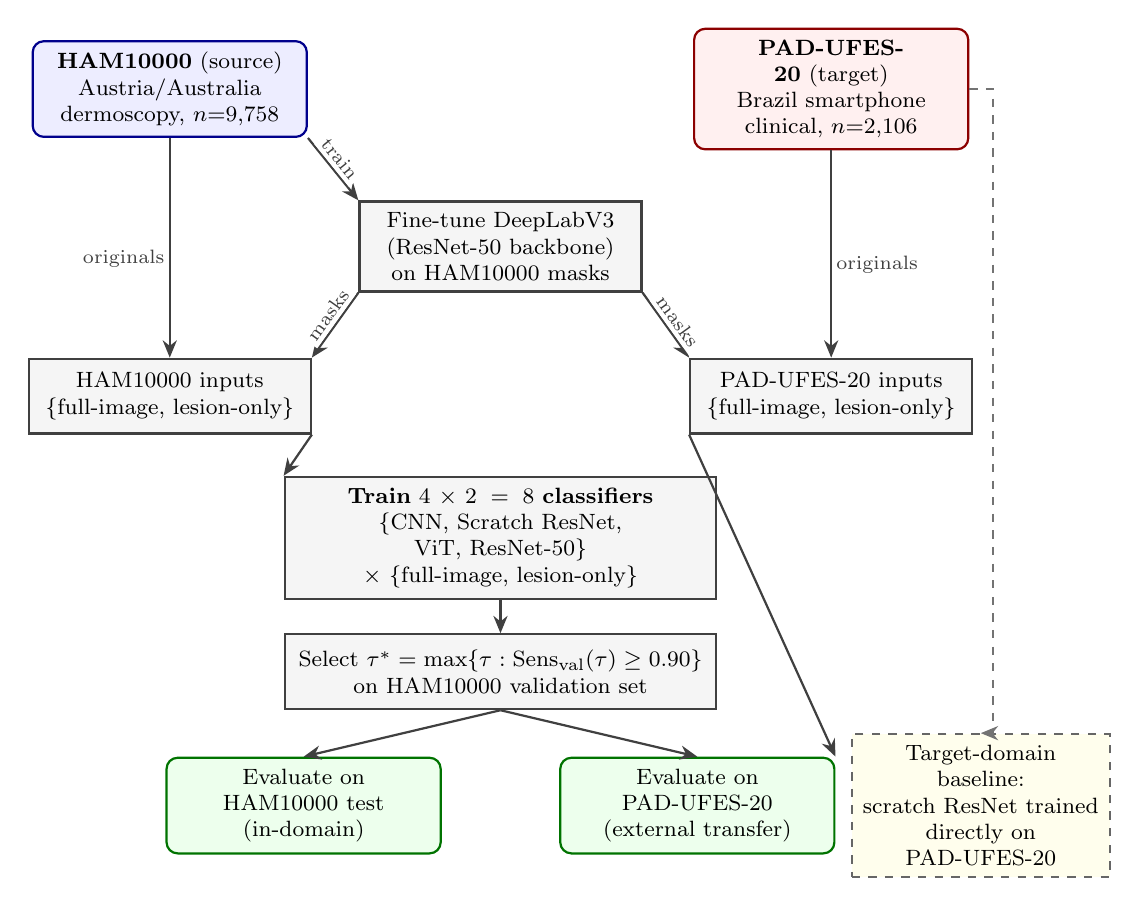
\begin{tikzpicture}[
        font=\footnotesize,
        every node/.style={align=center},
        source/.style={rectangle, rounded corners=4pt, draw=blue!55!black,
                       fill=blue!7, thick, minimum height=0.95cm,
                       inner sep=4pt, text width=3.2cm},
        target/.style={rectangle, rounded corners=4pt, draw=red!55!black,
                       fill=red!6, thick, minimum height=0.95cm,
                       inner sep=4pt, text width=3.2cm},
        process/.style={rectangle, draw=black!75, fill=gray!8,
                        thick, minimum height=0.95cm,
                        inner sep=4pt, text width=3.3cm},
        eval/.style={rectangle, rounded corners=4pt, draw=green!45!black,
                     fill=green!7, thick, minimum height=0.95cm,
                     inner sep=4pt, text width=3.2cm},
        baseline/.style={rectangle, dashed, draw=black!60, fill=yellow!7,
                         thick, minimum height=0.95cm,
                         inner sep=4pt, text width=3.0cm},
        arrow/.style={-{Stealth[length=2.2mm, width=1.8mm]}, thick, black!75},
        dasharrow/.style={-{Stealth[length=2.2mm, width=1.8mm]}, thick, dashed, black!55},
        arrlbl/.style={font=\scriptsize, inner sep=1.5pt, fill=white}
    ]
        % Row 1: Datasets
        \node[source] (ham) at (0,0) {\textbf{HAM10000} (source)\\Austria/Australia\\dermoscopy, $n{=}9{,}758$};
        \node[target] (pad) at (8.4,0) {\textbf{PAD-UFES-20} (target)\\Brazil smartphone\\clinical, $n{=}2{,}106$};

        % Center: DeepLabV3 segmentation (trained on HAM10000), feeds masks to both inputs
        \node[process] (seg) at (4.2,-2.0) {Fine-tune DeepLabV3\\(ResNet-50 backbone)\\on HAM10000 masks};

        % Row 2: Classifier inputs (under each dataset)
        \node[process] (ham_in) at (0,-3.9) {HAM10000 inputs\\\{full-image, lesion-only\}};
        \node[process] (pad_in) at (8.4,-3.9) {PAD-UFES-20 inputs\\\{full-image, lesion-only\}};

        % Row 3: Classifier training (only HAM10000 inputs)
        \node[process, text width=5.2cm] (train) at (4.2,-5.7)
            {\textbf{Train $4 \times 2 = 8$ classifiers}\\
             \{CNN, Scratch ResNet, ViT, ResNet-50\}\\
             $\times$ \{full-image, lesion-only\}};

        % Row 4: Threshold selection on HAM10000 validation
        \node[process, text width=5.2cm] (thresh) at (4.2,-7.4)
            {Select $\tau^{*} = \max\{\tau : \mathrm{Sens}_{\mathrm{val}}(\tau) \geq 0.90\}$\\
             on HAM10000 validation set};

        % Row 5: Evaluations
        \node[eval] (eham) at (1.7,-9.1) {Evaluate on\\HAM10000 test\\(in-domain)};
        \node[eval] (epad) at (6.7,-9.1) {Evaluate on\\PAD-UFES-20\\(external transfer)};

        % Target-domain baseline (separate path, not part of transfer eval)
        \node[baseline] (padbase) at (10.3,-9.1)
            {Target-domain baseline:\\scratch ResNet trained\\directly on PAD-UFES-20};

        % --- Arrows ---
        % HAM10000 supplies originals to its inputs and training data to the segmentation model
        \draw[arrow] (ham.south) -- node[arrlbl, left, pos=0.55] {originals} (ham_in.north);
        \draw[arrow] (ham.south east) -- node[arrlbl, sloped, above, pos=0.45] {train} (seg.north west);
        % DeepLabV3 masks feed the lesion-only variant for both datasets
        \draw[arrow] (seg.south west) -- node[arrlbl, sloped, above, pos=0.45] {masks} (ham_in.north east);
        \draw[arrow] (seg.south east) -- node[arrlbl, sloped, above, pos=0.55] {masks} (pad_in.north west);
        % PAD-UFES-20 supplies originals to its inputs
        \draw[arrow] (pad.south) -- node[arrlbl, right, pos=0.55] {originals} (pad_in.north);

        % Training pipeline: only HAM10000 inputs train the classifiers
        \draw[arrow] (ham_in.south east) -- (train.north west);
        \draw[arrow] (train.south) -- (thresh.north);

        % Threshold splits into two evaluations
        \draw[arrow] (thresh.south) -- (eham.north);
        \draw[arrow] (thresh.south) -- (epad.north);

        % PAD-UFES-20 inputs feed the PAD evaluation
        \draw[arrow] (pad_in.south west) -- (epad.north east);

        % Target-domain baseline: PAD-UFES-20 is also used to train a separate ResNet
        \draw[dasharrow] (pad.east) -- ++(0.3,0) |- (padbase.north);
    \end{tikzpicture}

    \vspace{4pt}
    \begin{minipage}{\linewidth}
        \footnotesize \emph{Notes:} Blue nodes denote source data; red nodes denote external target data; gray nodes denote modeling stages; green nodes denote evaluations. Each dataset contributes \emph{originals} (its raw images) to its own input box, which holds two classifier-input variants: \emph{full-image} (the originals) and \emph{lesion-only} (originals composited over white using a DeepLabV3 mask). DeepLabV3 is fine-tuned only on HAM10000, and only HAM10000 inputs are used to train classifiers, so the eight HAM10000-trained classifiers never see PAD-UFES-20 labels. The dashed yellow path is a separate target-domain baseline trained directly on PAD-UFES-20; it is shown only as a difficulty reference and is not part of the transfer evaluation.
    \end{minipage}
\end{figure}

\subsection{Lesion-Only Image Construction}

We create lesion-only images by predicting a binary lesion mask and compositing the original RGB image over a white background. Formally, for image $x$ and binary mask $m$, the transformed image is
\[
    \tilde{x}_{ijk} = m_{ij}\, x_{ijk} + (1-m_{ij}) \cdot 255.
\]
This transformation preserves the original lesion appearance and image geometry while suppressing pixels outside the predicted lesion region. We use the same procedure for HAM10000 and PAD-UFES-20. Thus the PAD-UFES-20 lesion-only images are generated without training a segmentation model on PAD-UFES-20 labels. We do approach this task in this way to mirror the fact that we want to study generalizability in the absence of (good) clinical training data.

We first trained a scratch segmentation baseline using binary lesion-mask supervision. This model was a simple U-Net with three downsampling stages of channel widths 32, 64, and 128, followed by a 256-channel bottleneck and a symmetric decoder with transposed-convolution upsampling and skip connections. Each convolutional block used two $3\times3$ convolutions with batch normalization and ReLU activations. We trained the model on the ISIC 2018 Task 1 lesion-boundary masks that correspond to our HAM10000 images, resizing inputs to $256\times256$, using batch size 16, Adam with learning rate $10^{-3}$, and a binary cross-entropy plus Dice loss objective. The predicted probability maps were thresholded at 0.5. This cutoff was selected using the validation set. At inference time, we retained the largest connected foreground component and filled holes, enforcing the prior that the primary lesion should form a single contiguous region. This scratch model reached a validation Dice score of approximately $0.786$ after post-processing. Qualitatively, it usually localized the main lesion, but it sometimes produced masks that were too small, too large, or failed on low-contrast cases. Because these segmentation errors would directly affect the lesion-only classifier inputs, we used a stronger segmentation model for the operational pipeline.

The operational lesion-only pipeline uses a pretrained DeepLabV3 model with a ResNet-50 backbone. We fine-tune it at $320\times320$ resolution with horizontal and vertical flips, right-angle rotations, color jitter, a binary cross-entropy plus Dice loss objective, AdamW with learning rate $10^{-4}$ and weight decay $10^{-4}$, cosine learning-rate decay, and early stopping on validation Dice. The best validation checkpoint reaches test Dice $0.909$ and test IoU $0.857$. We use this fine-tuned segmentation model to generate the masks used for all lesion-only classifier experiments.

\subsection{Classifier Families}

We train four classifiers on each input representation, giving eight HAM10000-trained models in total. The \emph{basic CNN} has four convolutional blocks with channels 32, 64, 128, and 256, followed by adaptive average pooling and a two-layer classifier. The \emph{scratch ResNet} uses a small residual architecture \cite{he2016resnet} with four stages, two residual blocks per stage, and channels 32, 64, 128, and 256. The \emph{vision transformer} \cite{dosovitskiy2021vit} uses $16\times16$ patches, embedding dimension 192, six transformer layers, six attention heads, and an MLP width of 384. The \emph{pretrained model} is a torchvision ResNet-50 initialized from ImageNet \cite{deng2009imagenet}; we first train the final linear head and then unfreeze layer~4 from epoch~6 onward, using a smaller learning rate for the unfrozen backbone.

We also report a simple \emph{mean ensemble} on PAD-UFES-20 that averages the four classifiers' malignant probabilities under each input representation. The ensemble uses the threshold corresponding to the same target sensitivity (see below), computed on the HAM10000 validation set from the averaged probabilities.

\subsection{Training and Model Selection}

All classifiers receive $224\times224$ RGB inputs normalized with ImageNet means and standard deviations. During training we use resize, random resized crop, horizontal and vertical flips, rotation, affine translation and scale, mild shear, mild perspective distortion, color jitter, occasional grayscale, and mild Gaussian blur. We train with AdamW, weight decay $10^{-4}$, batch size 32, cosine learning-rate decay, and at most 60 epochs. Key per-architecture choices are summarized in Table \ref{tab:hparams}.

\begin{table}[t]
    \centering
    \begin{threeparttable}
    \caption{Key training settings per classifier family.}
    \label{tab:hparams}
    \small
    \begin{tabular}{lcccc}
        \toprule
        Model & Head LR & Backbone LR & Unfreeze epoch & Notes \\
        \midrule
        Basic CNN & $3\times10^{-4}$ & --- & --- & 4 conv blocks, channels 32--256 \\
        Scratch ResNet & $3\times10^{-4}$ & --- & --- & 4 stages, 2 blocks/stage \\
        ViT & $2\times10^{-4}$ & --- & --- & patch 16, dim 192, 6 layers, 6 heads \\
        ImageNet ResNet-50 & $1\times10^{-3}$ & $1\times10^{-5}$ & 6 & head-only first, then layer~4 \\
        \bottomrule
    \end{tabular}
    \begin{tablenotes}[para]
        \footnotesize
        \item \emph{Notes:} All models share batch size 32, AdamW with weight decay $10^{-4}$, cosine learning-rate decay, up to 60 epochs, $224\times224$ inputs, and ImageNet normalization. The ResNet-50 head is trained first; layer~4 is unfrozen at epoch~6 with a smaller backbone learning rate.
    \end{tablenotes}
    \end{threeparttable}
\end{table}

We optimize weighted binary cross-entropy on logits. Because malignant and benign labels are imbalanced, we weight positive examples by the benign-to-malignant ratio in the training set:
\[
    \ell(f(x), y) =
    -\, w\, y \log \sigma(f(x)) \;-\; (1-y)\log(1-\sigma(f(x))),
\]
where $y=1$ denotes malignant and $w = N_{\text{benign}}/N_{\text{malignant}}$.

After each epoch we compute malignant probabilities on the validation set and choose the highest threshold whose validation sensitivity is at least 0.90:
\[
    \tau^* \;=\; \max \{\, \tau : \mathrm{Sens}_{\mathrm{val}}(\tau) \geq 0.90 \,\}.
\]
Sensitivity is $TP/(TP+FN)$ and specificity is $TN/(TN+FP)$. The implementation scans empirical score thresholds and keeps the most specific operating point that reaches the target. Since sensitivity and specificity are monotone step functions of the threshold, this is the highest qualifying threshold up to ties. We save a checkpoint whenever validation specificity improves while keeping sensitivity at the target. Training stops if no checkpoint improves for 20 epochs. We then reload the best checkpoint, recompute the validation threshold, and evaluate the model on the HAM10000 test set and on PAD-UFES-20 using that same threshold. Importantly, we do not tune thresholds on PAD-UFES-20 for the transfer evaluation.

For uncertainty, we bootstrap image-level predictions 5{,}000 times and report percentile 95\% confidence intervals for sensitivity and specificity. The bootstrap is applied to the saved prediction files, so it reflects sampling uncertainty conditional on each trained model and threshold. It does not include variation across random initializations.

\section{Empirical Contribution}

The main contribution is a controlled empirical test of whether lesion localization improves generalization. We compare each architecture against itself under two input representations, while holding the dataset split, label mapping, optimizer, data augmentation, threshold rule, and evaluation code fixed. This design isolates the effect of the lesion-only transformation more cleanly than a comparison across unrelated published models would.

The paper also contributes an external-domain evaluation. Within-dataset test accuracy can overstate practical usefulness when the train and test images share acquisition conditions. We therefore ask whether the HAM10000-selected thresholds transfer to PAD-UFES-20, whose images are Brazilian smartphone photographs rather than Austrian/Australian dermoscopic images and whose class distribution is very different. This is the more demanding test.

Finally, we include a target-domain baseline by training a scratch ResNet directly on PAD-UFES-20. This baseline does not answer the same question as the transfer experiment, because it is trained on PAD-UFES-20 rather than HAM10000, but it gives useful context. In particular, if a model trained on the target domain performs much better than the transferred models, the central bottleneck is likely domain shift rather than architecture alone.

\section{Results and Discussion}

\subsection{HAM10000 In-Domain Results}

Table \ref{tab:ham_results} reports held-out HAM10000 test performance, and Figure \ref{fig:performance_ci} visualizes the same sensitivity-specificity tradeoffs alongside the PAD-UFES-20 transfer results. Lesion-only inputs generally increase sensitivity relative to full-image inputs. The effect is largest for the CNN, where sensitivity rises from $0.836$ to $0.911$, and smallest for the ViT, where sensitivity rises only from $0.843$ to $0.863$. This pattern is consistent with the intended intervention, i.e. when background pixels are removed, the classifier flags malignancy more often.

\begin{figure}[t]
    \caption{Sensitivity and specificity for matched full-image and lesion-only classifiers.}
    \label{fig:performance_ci}
    \centering
    
\includegraphics[width=\linewidth]{performance_ci_ham_pad.pdf}

    \vspace{4pt}
    \begin{minipage}{\linewidth}
        \footnotesize \emph{Notes:} Columns separate held-out HAM10000 testing from PAD-UFES-20 external transfer; rows separate sensitivity and specificity. All points use the highest HAM10000 validation threshold that attains sensitivity at least 0.90. Error bars are image-level percentile 95\% bootstrap confidence intervals; the dashed line marks the 0.90 sensitivity target.
    \end{minipage}
\end{figure}

\begin{table}[t]
    \centering
    \begin{threeparttable}
    \caption{HAM10000 test performance.}
    \label{tab:ham_results}
    \footnotesize
    \begin{tabular}{llcccc}
        \toprule
        Model & Input & Sensitivity & Sens.\ CI & Specificity & Spec.\ CI \\
        \midrule
        CNN & full-image & 0.836 & [0.794, 0.879] & 0.727 & [0.701, 0.752] \\
        CNN & lesion-only & 0.911 & [0.877, 0.943] & 0.693 & [0.667, 0.720] \\
        Scratch ResNet & full-image & 0.887 & [0.848, 0.922] & 0.686 & [0.659, 0.712] \\
        Scratch ResNet & lesion-only & 0.911 & [0.877, 0.943] & 0.673 & [0.646, 0.701] \\
        ViT & full-image & 0.843 & [0.802, 0.884] & 0.726 & [0.700, 0.751] \\
        ViT & lesion-only & 0.863 & [0.822, 0.902] & 0.681 & [0.653, 0.707] \\
        ImageNet ResNet-50 & full-image & 0.846 & [0.804, 0.885] & 0.815 & [0.792, 0.837] \\
        ImageNet ResNet-50 & lesion-only & 0.877 & [0.838, 0.913] & 0.801 & [0.778, 0.824] \\
        \bottomrule
    \end{tabular}
    \begin{tablenotes}[para]
        \footnotesize
        \item \emph{Notes:} Thresholds are the highest HAM10000 validation thresholds that attain sensitivity at least 0.90. Brackets report 95\% bootstrap confidence intervals over images.
    \end{tablenotes}
    \end{threeparttable}
\end{table}

The specificity results are more mixed. In-domain, full-image models often retain slightly higher specificity, especially for the CNN, scratch ResNet, and ViT. The pretrained ResNet-50 is the strongest in-domain model by specificity under both input types.\footnote{Note that clinically deployed skin lesion classifiers tend to have relatively low specificity at around 95\% sensitivity. DermaSensor, a device for non-dermatology physicians, attains 26.2\% specificity at 97\% sensitivity \cite{manolakos2024ess}. Skin Analytics DERM attains, for earlier versions, 40.7–49.4\% specificity at 96-100\% sensitivity in real-world deployment \cite{thomas2023derm}.} At first glance, this weakens the case for lesion-only preprocessing. However, the in-domain setting is also where background shortcuts are least likely to be penalized: HAM10000 train, validation, and test images come from the same dataset and acquisition regime. The more important question is hence what happens when the image distribution changes.

\subsection{PAD-UFES-20 External Transfer}

Table \ref{tab:pad_transfer} reports transfer to PAD-UFES-20. Here, none of the HAM10000-trained models maintain the target sensitivity of $0.90$. This is the central negative result of the study. Thresholds that are acceptable on HAM10000 do not transport cleanly from dermoscopic source images to Brazilian smartphone clinical photographs.

\begin{table}[t]
    \centering
    \begin{threeparttable}
    \caption{PAD-UFES-20 transfer performance for HAM10000-trained models.}
    \label{tab:pad_transfer}
    \footnotesize
    \begin{tabular}{llcccc}
        \toprule
        Model & Input & Sensitivity & Sens.\ CI & Specificity & Spec.\ CI \\
        \midrule
        CNN & full-image & 0.453 & [0.428, 0.477] & 0.785 & [0.749, 0.820] \\
        CNN & lesion-only & 0.505 & [0.480, 0.528] & 0.868 & [0.838, 0.899] \\
        Scratch ResNet & full-image & 0.444 & [0.420, 0.468] & 0.806 & [0.769, 0.840] \\
        Scratch ResNet & lesion-only & 0.503 & [0.479, 0.527] & 0.835 & [0.802, 0.867] \\
        ViT & full-image & 0.785 & [0.765, 0.805] & 0.476 & [0.431, 0.519] \\
        ViT & lesion-only & 0.746 & [0.726, 0.768] & 0.476 & [0.431, 0.520] \\
        ImageNet ResNet-50 & full-image & 0.622 & [0.598, 0.645] & 0.766 & [0.727, 0.805] \\
        ImageNet ResNet-50 & lesion-only & 0.669 & [0.646, 0.692] & 0.622 & [0.577, 0.665] \\
        Mean ensemble & full-image & 0.578 & [0.554, 0.602] & 0.829 & [0.794, 0.861] \\
        Mean ensemble & lesion-only & 0.635 & [0.611, 0.658] & 0.781 & [0.745, 0.817] \\
        \bottomrule
    \end{tabular}
    \begin{tablenotes}[para]
        \footnotesize
        \item \emph{Notes:} Thresholds are the HAM10000 validation thresholds from Table~\ref{tab:ham_results}; no PAD-UFES-20 labels are used for threshold tuning. Brackets report 95\% bootstrap confidence intervals over all 2{,}106 PAD-UFES-20 images.
    \end{tablenotes}
    \end{threeparttable}
\end{table}

Within that negative result, lesion-only inputs still show a consistent partial benefit. They improve PAD-UFES-20 sensitivity for the CNN, scratch ResNet, ImageNet ResNet-50, and ensemble. They also improve specificity for the CNN and scratch ResNet. The ViT is the exception. Its full-image version already predicts malignancy more often on PAD-UFES-20, producing higher sensitivity but low specificity, and lesion-only preprocessing does not improve this tradeoff.

The main interpretation is therefore not necessarily that lesion-only preprocessing solves domain shift but that it appears to move several models in the desired direction under a difficult shift in country, camera, and clinical imaging protocol, especially for simpler convolutional models. This speaks against the argument that the lesion-only intervention is uninformative, but it also shows that background removal alone cannot repair calibration when the target domain differs in acquisition mode and class composition. Figure \ref{fig:pad_operating_points} visualizes the resulting operating points on PAD-UFES-20.

\begin{figure}[t]
    \caption{PAD-UFES-20 sensitivity-specificity operating points.}
    \label{fig:pad_operating_points}
    \centering
    
\includegraphics[width=0.78\linewidth]{pad_transfer_operating_points.pdf}

    \vspace{4pt}
    \begin{minipage}{\linewidth}
        \footnotesize \emph{Notes:} Blue and red circles are HAM10000-trained models evaluated on PAD-UFES-20 using the HAM10000 validation threshold; gray arrows point from each full-image model to its lesion-only counterpart. The black diamond marks a scratch ResNet trained and tuned directly on PAD-UFES-20, shown only as target-domain context. The dashed line marks the 0.90 sensitivity target.
    \end{minipage}
\end{figure}

\subsection{PAD-UFES-20 Target-Domain Baseline}

The PAD-trained scratch ResNet gives additional context in terms of what is feasible, i.e. how much signal is (at least) present in the actual images. Trained and tuned directly on the PAD-UFES-20 split, it reaches sensitivity $0.898$ with specificity $0.611$ on the PAD-UFES-20 test set of 317 images, with bootstrap confidence intervals $[0.858, 0.934]$ for sensitivity and $[0.494, 0.722]$ for specificity. This baseline nearly recovers the target sensitivity, but it does so at modest specificity.

\begin{table}[t]
    \centering
    \begin{threeparttable}
    \caption{Target-domain PAD-UFES-20 baseline.}
    \label{tab:pad_baseline}
    \footnotesize
    \begin{tabular}{lccccc}
        \toprule
        Model & Input & Sensitivity & Sens.\ CI & Specificity & Spec.\ CI \\
        \midrule
        PAD-trained Scratch ResNet & full-image & 0.898 & [0.858, 0.934] & 0.611 & [0.494, 0.722] \\
        \bottomrule
    \end{tabular}
    \begin{tablenotes}[para]
        \footnotesize
        \item \emph{Notes:} This model is trained, tuned, and tested on the PAD-UFES-20 split, so it is not a transfer model. It provides a rough upper-context comparison for the difficulty of the target domain.
    \end{tablenotes}
    \end{threeparttable}
\end{table}

This comparison suggests that the PAD-UFES-20 distribution is learnable, but not by simply transferring HAM10000 thresholds. The direct PAD baseline sees the target-domain images during training and validation, and therefore learns an operating point adapted to PAD-UFES-20. The HAM10000-trained models do not have that advantage. Reassuringly, the lesion-only ensemble closes part of the transfer sensitivity gap relative to the full-image ensemble, but the remaining gap is large.

\section{Limitations}

We emphasize three limitations. First, the segmentation model may introduce its own domain shift. A mask predictor trained on HAM10000-style images may fail on smartphone clinical images, and any such failure is inherited by the lesion-only classifiers. Because our evaluation measures downstream classification rather than mask quality on PAD-UFES-20, the lesion-only results conflate the value of lesion localization with the robustness of the segmentation model. With more space, one of the next steps would have been to dig deeper into the performance of the mask predictor and analyze the whole extract-then-classify pipeline as one.

Second, our confidence intervals bootstrap images for fixed trained models. They quantify test-sample uncertainty, not training-run uncertainty. A stronger version of this study would train each model across several random seeds and report variability across runs.

Third, the binary label mapping is clinically coarse. Some labels in the malignant group differ in appearance and clinical urgency, and the PAD-UFES-20 class distribution is not representative of a broad screening population. We therefore interpret sensitivity and specificity as experimental metrics for this matched-label task, not as deployable clinical performance.

\section{Conclusion}

Our central question was whether lesion-focused inputs improve skin cancer classification under domain shift? Our answer is qualified. On HAM10000, lesion-only inputs tend to increase sensitivity but often trade off specificity. On PAD-UFES-20, lesion-only inputs improve sensitivity for most architectures and improve both sensitivity and specificity for the simpler CNN and scratch ResNet, but all HAM10000-trained models remain poorly calibrated relative to the desired $0.90$ sensitivity target. Taken together, the evidence suggests that lesion localization is a useful intervention against some background dependence, but it is not sufficient by itself. Robust medical image classification requires both lesion-focused representations and target-domain calibration.

\section{Code and Reproducibility}

The codebase contains data preparation scripts, model definitions, training scripts, PAD-UFES-20 evaluation, and bootstrap confidence intervals. The full cluster pipeline is launched with
\[
\texttt{sbatch submit/submit\_full\_pipeline.sh}.
\]
The saved result table used in this report is \path{metrics/classification_bootstrap_metrics.csv}; segmentation metrics are stored in \path{metrics/segmentation_deeplabv3_resnet50_metrics.csv}, and the rendered paper figures live in \path{figures/}. The scratch U-Net segmentation baseline described in the Approach is documented as runnable notebooks in \path{notebooks/}, backed by \path{src/segmentation_unet.py}. The README explains the repository layout and notes that the cluster scripts currently use absolute compute-cluster paths for data and run directories.

\section{Project Contributions}
\begin{itemize}
    \item \textbf{Tobias Roemer} implemented and trained the full image and lesion-only classification models and evaluated on HAM10000 data.
    \item \textbf{Thomas Lee} performed transfer analysis and computed sensitivity, specificity, and class-wise metrics, and created the results tables.
    \item \textbf{Zichuan (Leo) Li} worked on the masking models and data preprocessing.
\end{itemize}
All authors contributed to experimental design, interpretation of results, manuscript editing, and final review.

\begin{thebibliography}{99}

\bibitem{chen2017deeplabv3}
Liang-Chieh Chen, George Papandreou, Florian Schroff, and Hartwig Adam.
\newblock Rethinking atrous convolution for semantic image segmentation.
\newblock \emph{arXiv preprint arXiv:1706.05587}, 2017.
\newblock \url{https://arxiv.org/abs/1706.05587}.

\bibitem{deng2009imagenet}
Jia Deng, Wei Dong, Richard Socher, Li-Jia Li, Kai Li, and Li Fei-Fei.
\newblock ImageNet: A large-scale hierarchical image database.
\newblock In \emph{IEEE Conference on Computer Vision and Pattern Recognition}, 2009.
\newblock \url{https://doi.org/10.1109/CVPR.2009.5206848}.

\bibitem{dosovitskiy2021vit}
Alexey Dosovitskiy, Lucas Beyer, Alexander Kolesnikov, Dirk Weissenborn, Xiaohua Zhai, Thomas Unterthiner, Mostafa Dehghani, Matthias Minderer, Georg Heigold, Sylvain Gelly, Jakob Uszkoreit, and Neil Houlsby.
\newblock An image is worth 16x16 words: Transformers for image recognition at scale.
\newblock In \emph{International Conference on Learning Representations}, 2021.
\newblock \url{https://openreview.net/forum?id=YicbFdNTTy}.

\bibitem{esteva2017dermatologist}
Andre Esteva, Brett Kuprel, Roberto A. Novoa, Justin Ko, Susan M. Swetter, Helen M. Blau, and Sebastian Thrun.
\newblock Dermatologist-level classification of skin cancer with deep neural networks.
\newblock \emph{Nature}, 542:115--118, 2017.
\newblock \url{https://doi.org/10.1038/nature21056}.

\bibitem{geirhos2020shortcut}
Robert Geirhos, J{\"o}rn-Henrik Jacobsen, Claudio Michaelis, Richard Zemel, Wieland Brendel, Matthias Bethge, and Felix A. Wichmann.
\newblock Shortcut learning in deep neural networks.
\newblock \emph{Nature Machine Intelligence}, 2:665--673, 2020.
\newblock \url{https://doi.org/10.1038/s42256-020-00257-z}.

\bibitem{he2016resnet}
Kaiming He, Xiangyu Zhang, Shaoqing Ren, and Jian Sun.
\newblock Deep residual learning for image recognition.
\newblock In \emph{IEEE Conference on Computer Vision and Pattern Recognition}, 2016.
\newblock \url{https://doi.org/10.1109/CVPR.2016.90}.

\bibitem{pacheco2020padufes20}
Andre G. C. Pacheco, Gustavo R. Lima, Amanda S. Salomao, Breno Krohling, Igor P. Biral, Gabriel G. de Angelo, F{\'a}bio C. R. Alves Jr., Jos{\'e} G. R. Esgario, Alana C. Simora, Pedro B. C. Castro, Filipe B. Rodrigues, and Renato A. Krohling.
\newblock PAD-UFES-20: A skin lesion dataset composed of patient data and clinical images collected from smartphones.
\newblock \emph{Data in Brief}, 32:106221, 2020.
\newblock \url{https://doi.org/10.1016/j.dib.2020.106221}.

\bibitem{ronneberger2015unet}
Olaf Ronneberger, Philipp Fischer, and Thomas Brox.
\newblock U-Net: Convolutional networks for biomedical image segmentation.
\newblock In \emph{Medical Image Computing and Computer-Assisted Intervention}, 2015.
\newblock \url{https://arxiv.org/abs/1505.04597}.

\bibitem{tschandl2018ham10000}
Philipp Tschandl, Cliff Rosendahl, and Harald Kittler.
\newblock The HAM10000 dataset, a large collection of multi-source dermatoscopic images of common pigmented skin lesions.
\newblock \emph{Scientific Data}, 5:180161, 2018.
\newblock \url{https://doi.org/10.1038/sdata.2018.161}.

\bibitem{manolakos2024ess}
Dimitris Manolakos, Daniel Gareau, Kristen M. Kelly, Waqas R. Farooq, Michael A. Marchetti, Anthony M. Rossi, Ashfaq A. Marghoob, and John A. Carucci.
\newblock Use of an elastic-scattering spectroscopy and artificial intelligence device in the detection of skin cancer.
\newblock \emph{JAAD International}, 14:129--138, 2024.
\newblock \url{https://doi.org/10.1016/j.jdin.2023.11.008}.

\bibitem{thomas2023derm}
Lucy Thomas, Chris Hyde, Dan Mullarkey, Jack Greenhalgh, Dilraj Kalsi, and Justin Ko.
\newblock Real-world post-deployment performance of a novel machine learning-based digital health technology for skin lesion assessment and suggestions for post-market surveillance.
\newblock \emph{Frontiers in Medicine}, 10:1264846, 2023.
\newblock \url{https://doi.org/10.3389/fmed.2023.1264846}.

\end{thebibliography}

\end{document}